\chapter{Peripherals}

All peripherals in \pulpino are connected to the APB bus, except the SPI slave
which is a very special peripheral and not intended to be used from the core
itself. See Chapter~\ref{chap:spi_slave} for details on the SPI slave.

\section{UART}

The UART used in this system is compatible with a 16750.
It features all the typical UART signals, see Table~\ref{tab:uart_signals}, plus
some additional signals defined by the 16750.

\begin{table}[H]
 \caption{External UART Signals}
 \label{tab:uart_signals}
  \begin{tabularx}{\textwidth}{@{}llX@{}} \toprule
    \textbf{Signal}   & \textbf{Direction} & \textbf{Description}         \\ \toprule
    \signal{uart\_tx}  & \textbf{output}    & Transmit Data                \\ \hline
    \signal{uart\_rx}  & \textbf{input}     & Receive Data                 \\ \hline
    \signal{uart\_rts} & \textbf{output}    & Request to Send              \\ \hline
    \signal{uart\_cts} & \textbf{input}     & Clear to send                \\ \hline
    \signal{uart\_dtr} & \textbf{output}    & Data Terminal Ready          \\ \hline
    \signal{uart\_dsr} & \textbf{input}     & Data Set Ready               \\ \hline
  \end{tabularx}
\end{table}


\clearpage
\section{GPIO}

\begin{table}[H]
 \caption{External GPIO Signals}
 \label{tab:gpio_signals}
  \begin{tabularx}{\textwidth}{@{}llX@{}} \toprule
    \textbf{Signal}                  & \textbf{Direction} & \textbf{Description}         \\ \toprule
    \signal{gpio\_in[31:0]}          & \textbf{input}     & Transmit Data                \\ \hline
    \signal{gpio\_out[31:0]}         & \textbf{output}    & Receive Data                 \\ \hline
    \signal{gpio\_dir[31:0]}         & \textbf{output}    & Request to Send              \\ \hline
    \signal{gpio\_padcfg[5:0][31:0]} & \textbf{output}    & Pad Configuration            \\ \hline
    \signal{interrupt}               & \textbf{output}    & Interrupt (Rise or Fall or Level)\\ \hline
  \end{tabularx}
\end{table}

\regDesc{0x1A10\_1000}{0x0000\_0000}{PADDIR (Pad Direction)}{
  \begin{bytefield}[rightcurly=.,endianness=big]{32}
  \bitheader{31,30,29,28,27,26,25,24,23,22,21,20,19,18,17,16,15,14,13,12,11,10,9,8,7,6,5,4,3,2,1,0} \\
  \begin{rightwordgroup}{PADDIR}
    \bitbox{1}{\tiny D}
    \bitbox{1}{\tiny D}
    \bitbox{1}{\tiny D}
    \bitbox{1}{\tiny D}
    \bitbox{1}{\tiny D}
    \bitbox{1}{\tiny D}
    \bitbox{1}{\tiny D}
    \bitbox{1}{\tiny D}
    \bitbox{1}{\tiny D}
    \bitbox{1}{\tiny D}
    \bitbox{1}{\tiny D}
    \bitbox{1}{\tiny D}
    \bitbox{1}{\tiny D}
    \bitbox{1}{\tiny D}
    \bitbox{1}{\tiny D}
    \bitbox{1}{\tiny D}
    \bitbox{1}{\tiny D}
    \bitbox{1}{\tiny D}
    \bitbox{1}{\tiny D}
    \bitbox{1}{\tiny D}
    \bitbox{1}{\tiny D}
    \bitbox{1}{\tiny D}
    \bitbox{1}{\tiny D}
    \bitbox{1}{\tiny D}
    \bitbox{1}{\tiny D}
    \bitbox{1}{\tiny D}
    \bitbox{1}{\tiny D}
    \bitbox{1}{\tiny D}
    \bitbox{1}{\tiny D}
    \bitbox{1}{\tiny D}
    \bitbox{1}{\tiny D}
    \bitbox{1}{\tiny D}
  \end{rightwordgroup}\\
  \end{bytefield}
}{
  \regItem{Bit 31:0}{PADDIR}{Pad Direction.\\
    Control the direction of each of the GPIO pads. A value of \signal{1} means
    it is configured as an output, while \signal{0} configures it as an input.
  }
}

\regDesc{0x1A10\_1004}{0x0000\_0000}{PADIN (Input Values)}{
  \begin{bytefield}[rightcurly=.,endianness=big]{32}
  \bitheader{31,30,29,28,27,26,25,24,23,22,21,20,19,18,17,16,15,14,13,12,11,10,9,8,7,6,5,4,3,2,1,0} \\
  \begin{rightwordgroup}{PADIN}
    \bitbox{1}{\tiny I}
    \bitbox{1}{\tiny I}
    \bitbox{1}{\tiny I}
    \bitbox{1}{\tiny I}
    \bitbox{1}{\tiny I}
    \bitbox{1}{\tiny I}
    \bitbox{1}{\tiny I}
    \bitbox{1}{\tiny I}
    \bitbox{1}{\tiny I}
    \bitbox{1}{\tiny I}
    \bitbox{1}{\tiny I}
    \bitbox{1}{\tiny I}
    \bitbox{1}{\tiny I}
    \bitbox{1}{\tiny I}
    \bitbox{1}{\tiny I}
    \bitbox{1}{\tiny I}
    \bitbox{1}{\tiny I}
    \bitbox{1}{\tiny I}
    \bitbox{1}{\tiny I}
    \bitbox{1}{\tiny I}
    \bitbox{1}{\tiny I}
    \bitbox{1}{\tiny I}
    \bitbox{1}{\tiny I}
    \bitbox{1}{\tiny I}
    \bitbox{1}{\tiny I}
    \bitbox{1}{\tiny I}
    \bitbox{1}{\tiny I}
    \bitbox{1}{\tiny I}
    \bitbox{1}{\tiny I}
    \bitbox{1}{\tiny I}
    \bitbox{1}{\tiny I}
    \bitbox{1}{\tiny I}
  \end{rightwordgroup}\\
  \end{bytefield}
}{
  \regItem{Bit 31:0}{PADIN}{Input Values.
  }
}

\regDesc{0x1A10\_1008}{0x0000\_0000}{PADOUT (Output Values)}{
  \begin{bytefield}[rightcurly=.,endianness=big]{32}
  \bitheader{31,30,29,28,27,26,25,24,23,22,21,20,19,18,17,16,15,14,13,12,11,10,9,8,7,6,5,4,3,2,1,0} \\
  \begin{rightwordgroup}{PADOUT}
    \bitbox{1}{\tiny O}
    \bitbox{1}{\tiny O}
    \bitbox{1}{\tiny O}
    \bitbox{1}{\tiny O}
    \bitbox{1}{\tiny O}
    \bitbox{1}{\tiny O}
    \bitbox{1}{\tiny O}
    \bitbox{1}{\tiny O}
    \bitbox{1}{\tiny O}
    \bitbox{1}{\tiny O}
    \bitbox{1}{\tiny O}
    \bitbox{1}{\tiny O}
    \bitbox{1}{\tiny O}
    \bitbox{1}{\tiny O}
    \bitbox{1}{\tiny O}
    \bitbox{1}{\tiny O}
    \bitbox{1}{\tiny O}
    \bitbox{1}{\tiny O}
    \bitbox{1}{\tiny O}
    \bitbox{1}{\tiny O}
    \bitbox{1}{\tiny O}
    \bitbox{1}{\tiny O}
    \bitbox{1}{\tiny O}
    \bitbox{1}{\tiny O}
    \bitbox{1}{\tiny O}
    \bitbox{1}{\tiny O}
    \bitbox{1}{\tiny O}
    \bitbox{1}{\tiny O}
    \bitbox{1}{\tiny O}
    \bitbox{1}{\tiny O}
    \bitbox{1}{\tiny O}
    \bitbox{1}{\tiny O}
  \end{rightwordgroup}\\
  \end{bytefield}
}{
  \regItem{Bit 31:0}{PADOUT}{Output Values.
  }
}

\regDesc{0x1A10\_100C}{0x0000\_0000}{INTEN (Interrupt Enable)}{
  \begin{bytefield}[rightcurly=.,endianness=big]{32}
  \bitheader{31,30,29,28,27,26,25,24,23,22,21,20,19,18,17,16,15,14,13,12,11,10,9,8,7,6,5,4,3,2,1,0} \\
  \begin{rightwordgroup}{INTEN}
    \bitbox{1}{\tiny IT}
    \bitbox{1}{\tiny IT}
    \bitbox{1}{\tiny IT}
    \bitbox{1}{\tiny IT}
    \bitbox{1}{\tiny IT}
    \bitbox{1}{\tiny IT}
    \bitbox{1}{\tiny IT}
    \bitbox{1}{\tiny IT}
    \bitbox{1}{\tiny IT}
    \bitbox{1}{\tiny IT}
    \bitbox{1}{\tiny IT}
    \bitbox{1}{\tiny IT}
    \bitbox{1}{\tiny IT}
    \bitbox{1}{\tiny IT}
    \bitbox{1}{\tiny IT}
    \bitbox{1}{\tiny IT}
    \bitbox{1}{\tiny IT}
    \bitbox{1}{\tiny IT}
    \bitbox{1}{\tiny IT}
    \bitbox{1}{\tiny IT}
    \bitbox{1}{\tiny IT}
    \bitbox{1}{\tiny IT}
    \bitbox{1}{\tiny IT}
    \bitbox{1}{\tiny IT}
    \bitbox{1}{\tiny IT}
    \bitbox{1}{\tiny IT}
    \bitbox{1}{\tiny IT}
    \bitbox{1}{\tiny IT}
    \bitbox{1}{\tiny IT}
    \bitbox{1}{\tiny IT}
    \bitbox{1}{\tiny IT}
    \bitbox{1}{\tiny IT}
  \end{rightwordgroup}\\
  \end{bytefield}
}{
  \regItem{Bit 31:0}{INTEN}{Interrupt Enable. \\
    Interrupt enable per input bit. INTTYPE0 and INTTYPE1 control the interrupt
    triggering behavior.

    There are four triggers available
    \begin{itemize}
      \item \signal{INTTYPE0 = 0, INTTYPE1 = 0}: Level 1
      \item \signal{INTTYPE0 = 1, INTTYPE1 = 0}: Level 0
      \item \signal{INTTYPE0 = 0, INTTYPE1 = 1}: Rise
      \item \signal{INTTYPE0 = 1, INTTYPE1 = 1}: Fall
    \end{itemize}
  }
}

\regDesc{0x1A10\_1010}{0x0000\_0000}{INTTYPE0 (Interrupt Type 0)}{
  \begin{bytefield}[rightcurly=.,endianness=big]{32}
  \bitheader{31,30,29,28,27,26,25,24,23,22,21,20,19,18,17,16,15,14,13,12,11,10,9,8,7,6,5,4,3,2,1,0} \\
  \begin{rightwordgroup}{INTTYPE0}
    \bitbox{1}{\tiny T0}
    \bitbox{1}{\tiny T0}
    \bitbox{1}{\tiny T0}
    \bitbox{1}{\tiny T0}
    \bitbox{1}{\tiny T0}
    \bitbox{1}{\tiny T0}
    \bitbox{1}{\tiny T0}
    \bitbox{1}{\tiny T0}
    \bitbox{1}{\tiny T0}
    \bitbox{1}{\tiny T0}
    \bitbox{1}{\tiny T0}
    \bitbox{1}{\tiny T0}
    \bitbox{1}{\tiny T0}
    \bitbox{1}{\tiny T0}
    \bitbox{1}{\tiny T0}
    \bitbox{1}{\tiny T0}
    \bitbox{1}{\tiny T0}
    \bitbox{1}{\tiny T0}
    \bitbox{1}{\tiny T0}
    \bitbox{1}{\tiny T0}
    \bitbox{1}{\tiny T0}
    \bitbox{1}{\tiny T0}
    \bitbox{1}{\tiny T0}
    \bitbox{1}{\tiny T0}
    \bitbox{1}{\tiny T0}
    \bitbox{1}{\tiny T0}
    \bitbox{1}{\tiny T0}
    \bitbox{1}{\tiny T0}
    \bitbox{1}{\tiny T0}
    \bitbox{1}{\tiny T0}
    \bitbox{1}{\tiny T0}
    \bitbox{1}{\tiny T0}
  \end{rightwordgroup}\\
  \end{bytefield}
}{
  \regItem{Bit 31:0}{INTTYPE0}{Interrupt Type 0. \\
    Controls the interrupt trigger behavior together with INTTYPE1. Use INTEN to
    enable interrupts first.
  }
}

\regDesc{0x1A10\_1014}{0x0000\_0000}{INTTYPE1 (Interrupt Type 1)}{
  \begin{bytefield}[rightcurly=.,endianness=big]{32}
  \bitheader{31,30,29,28,27,26,25,24,23,22,21,20,19,18,17,16,15,14,13,12,11,10,9,8,7,6,5,4,3,2,1,0} \\
  \begin{rightwordgroup}{INTTYPE1}
    \bitbox{1}{\tiny T1}
    \bitbox{1}{\tiny T1}
    \bitbox{1}{\tiny T1}
    \bitbox{1}{\tiny T1}
    \bitbox{1}{\tiny T1}
    \bitbox{1}{\tiny T1}
    \bitbox{1}{\tiny T1}
    \bitbox{1}{\tiny T1}
    \bitbox{1}{\tiny T1}
    \bitbox{1}{\tiny T1}
    \bitbox{1}{\tiny T1}
    \bitbox{1}{\tiny T1}
    \bitbox{1}{\tiny T1}
    \bitbox{1}{\tiny T1}
    \bitbox{1}{\tiny T1}
    \bitbox{1}{\tiny T1}
    \bitbox{1}{\tiny T1}
    \bitbox{1}{\tiny T1}
    \bitbox{1}{\tiny T1}
    \bitbox{1}{\tiny T1}
    \bitbox{1}{\tiny T1}
    \bitbox{1}{\tiny T1}
    \bitbox{1}{\tiny T1}
    \bitbox{1}{\tiny T1}
    \bitbox{1}{\tiny T1}
    \bitbox{1}{\tiny T1}
    \bitbox{1}{\tiny T1}
    \bitbox{1}{\tiny T1}
    \bitbox{1}{\tiny T1}
    \bitbox{1}{\tiny T1}
    \bitbox{1}{\tiny T1}
    \bitbox{1}{\tiny T1}
  \end{rightwordgroup}\\
  \end{bytefield}
}{
  \regItem{Bit 31:0}{INTTYPE1}{Interrupt Type 1. \\
    Controls the interrupt trigger behavior together with INTTYPE0. Use INTEN to
    enable interrupts first.
  }
}

\regDesc{0x1A10\_1018}{0x0000\_0000}{INTSTATUS (Interrupt Status)}{
  \begin{bytefield}[rightcurly=.,endianness=big]{32}
  \bitheader{31,30,29,28,27,26,25,24,23,22,21,20,19,18,17,16,15,14,13,12,11,10,9,8,7,6,5,4,3,2,1,0} \\
  \begin{rightwordgroup}{INTSTATUS}
    \bitbox{1}{\tiny S}
    \bitbox{1}{\tiny S}
    \bitbox{1}{\tiny S}
    \bitbox{1}{\tiny S}
    \bitbox{1}{\tiny S}
    \bitbox{1}{\tiny S}
    \bitbox{1}{\tiny S}
    \bitbox{1}{\tiny S}
    \bitbox{1}{\tiny S}
    \bitbox{1}{\tiny S}
    \bitbox{1}{\tiny S}
    \bitbox{1}{\tiny S}
    \bitbox{1}{\tiny S}
    \bitbox{1}{\tiny S}
    \bitbox{1}{\tiny S}
    \bitbox{1}{\tiny S}
    \bitbox{1}{\tiny S}
    \bitbox{1}{\tiny S}
    \bitbox{1}{\tiny S}
    \bitbox{1}{\tiny S}
    \bitbox{1}{\tiny S}
    \bitbox{1}{\tiny S}
    \bitbox{1}{\tiny S}
    \bitbox{1}{\tiny S}
    \bitbox{1}{\tiny S}
    \bitbox{1}{\tiny S}
    \bitbox{1}{\tiny S}
    \bitbox{1}{\tiny S}
    \bitbox{1}{\tiny S}
    \bitbox{1}{\tiny S}
    \bitbox{1}{\tiny S}
    \bitbox{1}{\tiny S}
  \end{rightwordgroup}\\
  \end{bytefield}
}{
  \regItem{Bit 31:0}{INTSTATUS}{Interrupt Status. \\
    Contains interrupt status per GPIO line. The status register is cleared when
    read. Similarly the \signal{interrupt} line is high while a bit is set in
    interrupt status and will be deasserted when the status register is read.
  }
}

\regDesc{0x1A10\_1020 - 0x1A10\_103C}{0x0000\_0000}{PADCFG0-7 (Pad Configuration
Registers 0-7)}{
  \begin{bytefield}[rightcurly=.,endianness=big]{32}
  \bitheader{31,30,29,28,27,26,25,24,23,22,21,20,19,18,17,16,15,14,13,12,11,10,9,8,7,6,5,4,3,2,1,0} \\
  \begin{rightwordgroup}{PADCFG0-7}
    \bitbox{1}{\tiny P}
    \bitbox{1}{\tiny P}
    \bitbox{1}{\tiny P}
    \bitbox{1}{\tiny P}
    \bitbox{1}{\tiny P}
    \bitbox{1}{\tiny P}
    \bitbox{1}{\tiny P}
    \bitbox{1}{\tiny P}
    \bitbox{1}{\tiny P}
    \bitbox{1}{\tiny P}
    \bitbox{1}{\tiny P}
    \bitbox{1}{\tiny P}
    \bitbox{1}{\tiny P}
    \bitbox{1}{\tiny P}
    \bitbox{1}{\tiny P}
    \bitbox{1}{\tiny P}
    \bitbox{1}{\tiny P}
    \bitbox{1}{\tiny P}
    \bitbox{1}{\tiny P}
    \bitbox{1}{\tiny P}
    \bitbox{1}{\tiny P}
    \bitbox{1}{\tiny P}
    \bitbox{1}{\tiny P}
    \bitbox{1}{\tiny P}
    \bitbox{1}{\tiny P}
    \bitbox{1}{\tiny P}
    \bitbox{1}{\tiny P}
    \bitbox{1}{\tiny P}
    \bitbox{1}{\tiny P}
    \bitbox{1}{\tiny P}
    \bitbox{1}{\tiny P}
    \bitbox{1}{\tiny P}
  \end{rightwordgroup}\\
  \end{bytefield}
}{
  \regItem{Bit 31:0}{PADCFG0-7}{Pad Configuration Registers. \\
    The pad configuration registers control various aspects of the pads that are
    typically used in ASICs, e.g. drive strength, Schmitt-Triggers, Slew Rate,
    etc. Since those configuration parameters depend on the exact pads used,
    each implementation is free to use the PADCFG0-7 registers in every way it
    wants and also leave them unconnected, if unneeded.
  }
}

\clearpage
\section{SPI Master}

\begin{table}[H]
 \caption{SPI Signals}
 \label{tab:spi_signals}
  \begin{tabularx}{\textwidth}{@{}llX@{}} \toprule
    \textbf{Signal}                  & \textbf{Direction} & \textbf{Description}        \\ \toprule
    \signal{spi\_clk}                & \textbf{output}    & Master Clock                \\ \hline
    \signal{spi\_csn0}               & \textbf{output}    & Chip Select 0               \\ \hline
    \signal{spi\_csn1}               & \textbf{output}    & Chip Select 1               \\ \hline
    \signal{spi\_csn2}               & \textbf{output}    & Chip Select 2               \\ \hline
    \signal{spi\_csn3}               & \textbf{output}    & Chip Select 3               \\ \hline
    \signal{spi\_mode[1:0]}          & \textbf{output}    & SPI Mode                    \\ \hline
    \signal{spi\_sdo0}               & \textbf{output}    & Output Line 0               \\ \hline
    \signal{spi\_sdo1}               & \textbf{output}    & Output Line 1               \\ \hline
    \signal{spi\_sdo2}               & \textbf{output}    & Output Line 2               \\ \hline
    \signal{spi\_sdo3}               & \textbf{output}    & Output Line 3               \\ \hline
    \signal{spi\_sdi0}               & \textbf{input}     & Input Line 0                \\ \hline
    \signal{spi\_sdi1}               & \textbf{input}     & Input Line 1                \\ \hline
    \signal{spi\_sdi2}               & \textbf{input}     & Input Line 2                \\ \hline
    \signal{spi\_sdi3}               & \textbf{input}     & Input Line 3                \\ \hline
    \signal{events\_o[1:0]}          & \textbf{output}    & Event/Interrupt             \\ \hline
  \end{tabularx}
\end{table}

\regDesc{0x1A10\_2000}{0x0000\_0000}{STATUS (Status Register)}{
  \begin{bytefield}[rightcurly=.,endianness=big]{32}
  \bitheader{31,11,8,5,4,3,2,1,0} \\
  \begin{rightwordgroup}{STATUS}
    \bitbox{20}{unused}
    \bitbox{4}{CS}
    \bitbox{3}{0}
    \bitbox{1}{\rotatebox{90}{\tiny SRST}}
    \bitbox{1}{\rotatebox{90}{\tiny QWR}}
    \bitbox{1}{\rotatebox{90}{\tiny QRD}}
    \bitbox{1}{\rotatebox{90}{\tiny WR}}
    \bitbox{1}{\rotatebox{90}{\tiny RD}}
  \end{rightwordgroup}\\
  \end{bytefield}
}{
  \regItem{Bit 11:8}{CS}{Chip Select.\\
    Specify the chip select signal that should be used for the next transfer.
  }
  \regItem{Bit 4}{SRST}{Software Reset.\\
    Clear FIFOs and abort active transfers.
  }
  \regItem{Bit 3}{QWR}{Quad Write Command.\\
    Perform a write using Quad SPI mode.
  }
  \regItem{Bit 2}{QRD}{Quad Read Command.\\
    Perform a read using Quad SPI mode.
  }
  \regItem{Bit 1}{WR}{Write Command.\\
    Perform a write using standard SPI mode.
  }
  \regItem{Bit 0}{RD}{Read Command.\\
    Perform a read using standard SPI mode.
  }
}

\regDesc{0x1A10\_2004}{0x0000\_0000}{CLKDIV (Clock Divider)}{
  \begin{bytefield}[rightcurly=.,endianness=big]{32}
  \bitheader{31,11,8,5,4,3,2,1,0} \\
  \begin{rightwordgroup}{CLKDIV}
    \bitbox{24}{unused}
    \bitbox{8}{CLKDIV}
  \end{rightwordgroup}\\
  \end{bytefield}
}{
  \regItem{Bit 7:0}{CLKDIV}{Clock Divider.\\
    Clock divider value used to divide the SoC clock for the SPI transfers. This
    register should not be modified while a transfer is in progress.
  }
}

\regDesc{0x1A10\_2008}{0x0000\_0000}{SPICMD (SPI Command)}{
  \begin{bytefield}[rightcurly=.,endianness=big]{32}
  \bitheader{31,0} \\
  \begin{rightwordgroup}{SPICMD}
    \bitbox{32}{SPICMD}
  \end{rightwordgroup}\\
  \end{bytefield}
}{
  \regItem{Bit 31:0}{SPICMD}{SPI Command.\\
    When performing a read or write transfer the SPI command is sent first
    before any data is read or written.
    The length of the SPI command can be controlled with the \signal{SPILEN}
    register.
  }
}

\regDesc{0x1A10\_200C}{0x0000\_0000}{SPIADR (SPI Address)}{
  \begin{bytefield}[rightcurly=.,endianness=big]{32}
  \bitheader{31,0} \\
  \begin{rightwordgroup}{SPIADR}
    \bitbox{32}{SPIADR}
  \end{rightwordgroup}\\
  \end{bytefield}
}{
  \regItem{Bit 31:0}{SPIADR}{SPI Address.\\
    When performing a read or write transfer the SPI command is sent first
    before any data is read or written, after this the SPI address is sent.
    The length of the SPI address can be controlled with the \signal{SPILEN}
    register.
  }
}

\regDesc{0x1A10\_2010}{0x0000\_0000}{SPILEN (SPI Transfer Length)}{
  \begin{bytefield}[rightcurly=.,endianness=big]{32}
  \bitheader{31,0} \\
  \begin{rightwordgroup}{SPILEN}
    \bitbox{16}{DATALEN}
    \bitbox{4}{0}
    \bitbox{6}{ADDRLEN}
    \bitbox{6}{CMDLEN}
  \end{rightwordgroup}\\
  \end{bytefield}
}{
  \regItem{Bit 31:16}{DATALEN}{SPI Data Length.\\
    The number of bits read or written.
    Note that first the SPI command and address are written to an SPI slave
    device.
  }
  \regItem{Bit 13:8}{ADDRLEN}{SPI Address Length.\\
    The number of bits of the SPI address that should be sent.
  }
  \regItem{Bit 5:0}{CMDLEN}{SPI Command Length.\\
    The number of bits of the SPI command that should be sent.
  }
}

\regDesc{0x1A10\_2014}{0x0000\_0000}{SPIDUM (SPI Dummy Cycles)}{
  \begin{bytefield}[rightcurly=.,endianness=big]{32}
  \bitheader{31,0} \\
  \begin{rightwordgroup}{SPIDUM}
    \bitbox{16}{DUMMYWR}
    \bitbox{16}{DUMMYRD}
  \end{rightwordgroup}\\
  \end{bytefield}
}{
  \regItem{Bit 31:16}{DUMMYWR}{Write Dummy Cycles.\\
    Dummy cycles (nothing being written or read) between sending the SPI
    command + SPI address and writing the data.
  }
  \regItem{Bit 15:0}{DUMMYRD}{Read Dummy Cycles.\\
    Dummy cycles (nothing being written or read) between sending the SPI
    command + SPI address and reading the data.
  }
}

\regDesc{0x1A10\_2018}{0x0000\_0000}{TXFIFO (SPI Transmit FIFO)}{
  \begin{bytefield}[rightcurly=.,endianness=big]{32}
  \bitheader{31,0} \\
  \begin{rightwordgroup}{TXFIFO}
    \bitbox{32}{TX}
  \end{rightwordgroup}\\
  \end{bytefield}
}{
  \regItem{Bit 31:0}{TX}{Transmit Data.\\
    Write data into the FIFO.
  }
}

\regDesc{0x1A10\_2020}{0x0000\_0000}{RXFIFO (SPI Receive FIFO)}{
  \begin{bytefield}[rightcurly=.,endianness=big]{32}
  \bitheader{31,0} \\
  \begin{rightwordgroup}{RXFIFO}
    \bitbox{32}{RX}
  \end{rightwordgroup}\\
  \end{bytefield}
}{
  \regItem{Bit 31:0}{RX}{Receive Data.\\
    Read data from the FIFO.
  }
}

\regDesc{0x1A10\_2024}{0x0000\_0000}{INTCFG (Interrupt Configuration)}{
  \begin{bytefield}[rightcurly=.,endianness=big]{32}
  \bitheader{31,0} \\
  \begin{rightwordgroup}{INTCFG}
    \bitbox{1}{\rotatebox{90}{\tiny EN}}
    \bitbox{1}{\rotatebox{90}{\tiny CNTEN}}
    \bitbox{2}{0}
    \bitbox{4}{CNTRX}
    \bitbox{4}{0}
    \bitbox{4}{CNTTX}
    \bitbox{4}{0}
    \bitbox{4}{RHTX}
    \bitbox{4}{0}
    \bitbox{4}{THTX}
  \end{rightwordgroup}\\
  \end{bytefield}
}{
  \regItem{Bit 31}{EN}{Interrupt Enable.\\
    Enable interrupts
  }
}

\clearpage
\section{I2C}

\regDesc{0x1A10\_5000}{0x0000\_0000}{CPR (Clock Prescale Register)}{
  \begin{bytefield}[rightcurly=.,endianness=big]{32}
  \bitheader{31,15,0} \\
  \begin{rightwordgroup}{CPR}
    \bitbox{16}{unused}
    \bitbox{16}{PRE}
  \end{rightwordgroup}\\
  \end{bytefield}
}{
  \regItem{Bit 15:0}{PRE}{Prescaler.\\
    Sets the clock prescaler by the value in PRE to
    achieve the desired I2C clock by dividing the current system clock by the
    given factor.}
}


\regDesc{0x1A10\_5004}{0x0000\_0000}{CTRL (Control Register)}{
  \begin{bytefield}[rightcurly=.,endianness=big]{32}
  \bitheader{31,15,0} \\
  \begin{rightwordgroup}{CTRL}
    \bitbox{24}{unused}
    \bitbox{1}{\rotatebox{90}{\tiny EN}}
    \bitbox{1}{\rotatebox{90}{\tiny IE}}
    \bitbox{1}{-}
    \bitbox{1}{-}
    \bitbox{1}{-}
    \bitbox{1}{-}
    \bitbox{1}{-}
    \bitbox{1}{-}
  \end{rightwordgroup}\\
  \end{bytefield}
}{
  \regItem{Bit 7}{EN}{Enable.\\
  Enable the I2C peripheral.}
  \regItem{Bit 6}{IE}{Interrupt enable.\\
  Enable interrupts.}
  \regItem{Bit 5:0}{Reserved}{Set to 0.}
}



\regDesc{0x1A10\_5008}{0x0000\_0000}{TX (Transmit Register)}{
  \begin{bytefield}[rightcurly=.,endianness=big]{32}
  \bitheader{31,15,0} \\
  \begin{rightwordgroup}{TX}
    \bitbox{24}{unused}
    \bitbox{8}{TX}
  \end{rightwordgroup}\\
  \end{bytefield}
}{
  \regItem{Bit 7:0}{TX}{Transmit Register}
}


\regDesc{0x1A10\_500C}{0x0000\_0000}{RX (Receive Register)}{
  \begin{bytefield}[rightcurly=.,endianness=big]{32}
  \bitheader{31,15,0} \\
  \begin{rightwordgroup}{TX}
    \bitbox{24}{unused}
    \bitbox{8}{RX}
  \end{rightwordgroup} \\
  \end{bytefield}
}
{
  \regItem{Bit 7:0}{RX}{Receive Register}
}


\regDesc{0x1A10\_5010}{0x0000\_0000}{CMD (Command Register)}{
  \begin{bytefield}[rightcurly=.,endianness=big]{32}
  \bitheader{31,15,0} \\
  \begin{rightwordgroup}{CMD}
    \bitbox{24}{unused}
    \bitbox{1}{\rotatebox{90}{\small \tiny STA}}
    \bitbox{1}{\rotatebox{90}{\small \tiny STO}}
    \bitbox{1}{\rotatebox{90}{\small \tiny RD}}
    \bitbox{1}{\rotatebox{90}{\small \tiny WR}}
    \bitbox{1}{\rotatebox{90}{\small \tiny ACK}}
    \bitbox{1}{0}
    \bitbox{1}{0}
    \bitbox{1}{\rotatebox{90}{\small \tiny IA}}
  \end{rightwordgroup}\\
  \end{bytefield}
}{
  \regItem{Bit 7}{STA}{Send start bit.}
  \regItem{Bit 6}{STO}{Send stop bit.}
  \regItem{Bit 5}{RD}{Read from bus.}
  \regItem{Bit 4}{WR}{Write to bus.}
  \regItem{Bit 3}{ACK}{Acknowledge received data.}
  \regItem{Bit 2:1}{Reserved}{Set to 0.}
  \regItem{Bit 0}{IA}{Interrupt Acknowldge.\\
    Set to one to acknowledge interrupt.
    Cleared when transmission is done or arbitration is lost.}
}


\regDesc{0x1A10\_5014}{0x0000\_0000}{STATUS (Status Register)}{
  \begin{bytefield}[rightcurly=.,endianness=big]{32}
  \bitheader{31,15,0} \\
  \begin{rightwordgroup}{STATUS}
    \bitbox{24}{unused}
    \bitbox{1}{\rotatebox{90}{\small \tiny RXA}}
    \bitbox{1}{\rotatebox{90}{\small \tiny BUS}}
    \bitbox{1}{\rotatebox{90}{\small \tiny AL}}
    \bitbox{1}{0}
    \bitbox{1}{0}
    \bitbox{1}{0}
    \bitbox{1}{\rotatebox{90}{\small \tiny TIP}}
    \bitbox{1}{\rotatebox{90}{\small \tiny IRQ}}
  \end{rightwordgroup}\\
  \end{bytefield}
}{
  \regItem{Bit 7}{RXA}{Acknowledge from sent data.}
  \regItem{Bit 6}{BUS}{Bus is busy.}
  \regItem{Bit 5}{AL}{Arbitration lost.}
  \regItem{Bit 4:2}{Reserved}{Set to 0.}
  \regItem{Bit 1}{TIP}{Transfer in progress.}
  \regItem{Bit 0}{IRQ}{Interrupt received.\\
    This flag is always set when transmission has finished or bus arpitration
  was lostm, regardless of whether interrupts are enabled or not. This flag can
possibly polled and is cleared by writing 1 to the IA command register.}
}


\clearpage
\section{Timer}

The timer unit has no external signals.

The timer unit has 2 timers per default. This can be overwritten by a parameter
when instantiating the timer.

\regDesc{0x1A10\_30?0}{0x0000\_0000}{TIMER (Current Timer Value)}{
  \begin{bytefield}[rightcurly=.,endianness=big]{32}
  \bitheader{31,15,0} \\
  \begin{rightwordgroup}{TIMER}
    \bitbox{32}{TIMER}
  \end{rightwordgroup}\\
  \end{bytefield}
}{
  \regItem{Bit 31:0}{TIMER}{Current Timer Value.\\
    Current value of the timer. There is an internal prescaler per timer that
    allows to specify the interval in which the timer will be increased. The
    prescaler is controlled by \signal{CTRL}.

    When \signal{TIMER} reaches \signal{FFFF\_FFFF} an interrupt will be
    raised.
  }
}

\regDesc{0x1A10\_30?4}{0x0000\_0000}{CTRL (Timer Control)}{
  \begin{bytefield}[rightcurly=.,endianness=big]{32}
  \bitheader{31,15,0} \\
  \begin{rightwordgroup}{CTRL}
    \bitbox{26}{unused}
    \bitbox{3}{\tiny PRE}
    \bitbox{2}{0}
    \bitbox{1}{\rotatebox{90}{\tiny EN}}
  \end{rightwordgroup}\\
  \end{bytefield}
}{
  \regItem{Bit 5:3}{PRE}{Prescaler value.}
  \regItem{Bit 0}{EN}{Enable the timer.}
}

\regDesc{0x1A10\_30?8}{0x0000\_0000}{CMP (Timer Compare)}{
  \begin{bytefield}[rightcurly=.,endianness=big]{32}
  \bitheader{31,15,0} \\
  \begin{rightwordgroup}{CMP}
    \bitbox{32}{CMP}
  \end{rightwordgroup}\\
  \end{bytefield}
}{
  \regItem{Bit 31:0}{CMP}{Timer Compare.\\
    An interrupt will be raised when \signal{TIMER} reaches \signal{CMP}
  }
}

\clearpage
\section{Event Unit}

\pulpino features a lightweight event and interrupt unit which supports
vectorized interrupts of up to 32 lines and event triggering of up to 32 input
lines. The interrupt and event lines are separately masked and buffered, see
Figure~\ref{fig:event_unit}.


\begin{figure}[H]
  \centering
  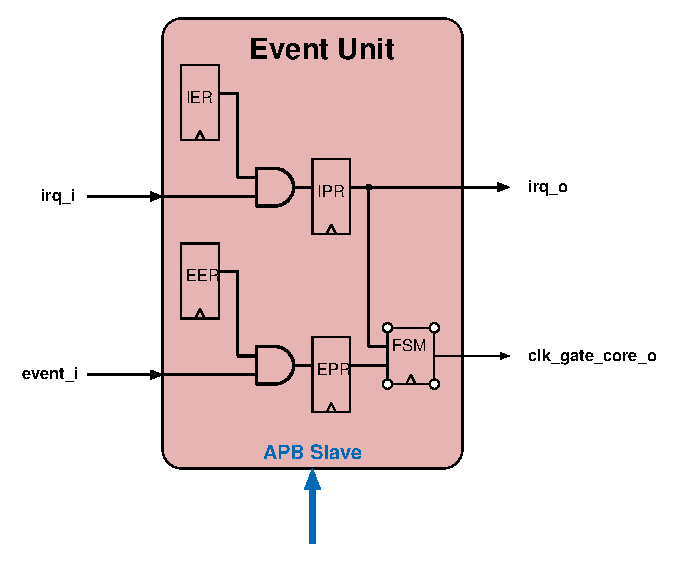
\includegraphics[width=0.6\textwidth]{./figures/event_unit}
  \caption{Event Unit.}
  \label{fig:event_unit}
\end{figure}

The current assignment of event and interrupt lines is given in
Figure~\ref{fig:event_lines}. Note that \signal{irq\_i} and \signal{event\_i}
are bound together.

\begin{figure}[H]
  \centering
  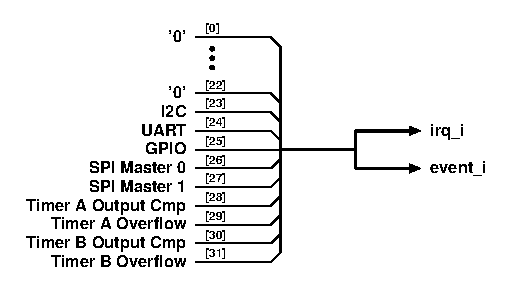
\includegraphics[width=0.6\textwidth]{./figures/event_lines}
  \caption{Event Lines.}
  \label{fig:event_lines}
\end{figure}


\regDesc{0x1A10\_4000}{0x0000\_0000}{IER (Interrupt Enable)}{
  \begin{bytefield}[rightcurly=.,endianness=big]{32}
  \bitheader{31,30,29,28,27,26,25,24,23,22,21,20,19,18,17,16,15,14,13,12,11,10,9,8,7,6,5,4,3,2,1,0} \\
  \begin{rightwordgroup}{IER}
    \bitbox{1}{\tiny E}
    \bitbox{1}{\tiny E}
    \bitbox{1}{\tiny E}
    \bitbox{1}{\tiny E}
    \bitbox{1}{\tiny E}
    \bitbox{1}{\tiny E}
    \bitbox{1}{\tiny E}
    \bitbox{1}{\tiny E}
    \bitbox{1}{\tiny E}
    \bitbox{1}{\tiny E}
    \bitbox{1}{\tiny E}
    \bitbox{1}{\tiny E}
    \bitbox{1}{\tiny E}
    \bitbox{1}{\tiny E}
    \bitbox{1}{\tiny E}
    \bitbox{1}{\tiny E}
    \bitbox{1}{\tiny E}
    \bitbox{1}{\tiny E}
    \bitbox{1}{\tiny E}
    \bitbox{1}{\tiny E}
    \bitbox{1}{\tiny E}
    \bitbox{1}{\tiny E}
    \bitbox{1}{\tiny E}
    \bitbox{1}{\tiny E}
    \bitbox{1}{\tiny E}
    \bitbox{1}{\tiny E}
    \bitbox{1}{\tiny E}
    \bitbox{1}{\tiny E}
    \bitbox{1}{\tiny E}
    \bitbox{1}{\tiny E}
    \bitbox{1}{\tiny E}
    \bitbox{1}{\tiny E}
  \end{rightwordgroup}\\
  \end{bytefield}
}{
  \regItem{Bit 31:0}{IER}{Interrupt Enable.\\
    Enable interrupts per line.
  }
}

\regDesc{0x1A10\_4004}{0x0000\_0000}{IPR (Interrupt Pending)}{
  \begin{bytefield}[rightcurly=.,endianness=big]{32}
  \bitheader{31,30,29,28,27,26,25,24,23,22,21,20,19,18,17,16,15,14,13,12,11,10,9,8,7,6,5,4,3,2,1,0} \\
  \begin{rightwordgroup}{IPR}
    \bitbox{1}{\tiny P}
    \bitbox{1}{\tiny P}
    \bitbox{1}{\tiny P}
    \bitbox{1}{\tiny P}
    \bitbox{1}{\tiny P}
    \bitbox{1}{\tiny P}
    \bitbox{1}{\tiny P}
    \bitbox{1}{\tiny P}
    \bitbox{1}{\tiny P}
    \bitbox{1}{\tiny P}
    \bitbox{1}{\tiny P}
    \bitbox{1}{\tiny P}
    \bitbox{1}{\tiny P}
    \bitbox{1}{\tiny P}
    \bitbox{1}{\tiny P}
    \bitbox{1}{\tiny P}
    \bitbox{1}{\tiny P}
    \bitbox{1}{\tiny P}
    \bitbox{1}{\tiny P}
    \bitbox{1}{\tiny P}
    \bitbox{1}{\tiny P}
    \bitbox{1}{\tiny P}
    \bitbox{1}{\tiny P}
    \bitbox{1}{\tiny P}
    \bitbox{1}{\tiny P}
    \bitbox{1}{\tiny P}
    \bitbox{1}{\tiny P}
    \bitbox{1}{\tiny P}
    \bitbox{1}{\tiny P}
    \bitbox{1}{\tiny P}
    \bitbox{1}{\tiny P}
    \bitbox{1}{\tiny P}
  \end{rightwordgroup}\\
  \end{bytefield}
}{
  \regItem{Bit 31:0}{IPR}{Interrupt Pending.\\
    Write/read pending interrupts per line.
  }
}

\regDesc{0x1A10\_4008}{0x0000\_0000}{ISP (Interrupt Set Pending)}{
  \begin{bytefield}[rightcurly=.,endianness=big]{32}
  \bitheader{31,30,29,28,27,26,25,24,23,22,21,20,19,18,17,16,15,14,13,12,11,10,9,8,7,6,5,4,3,2,1,0} \\
  \begin{rightwordgroup}{ISP}
    \bitbox{1}{\tiny S}
    \bitbox{1}{\tiny S}
    \bitbox{1}{\tiny S}
    \bitbox{1}{\tiny S}
    \bitbox{1}{\tiny S}
    \bitbox{1}{\tiny S}
    \bitbox{1}{\tiny S}
    \bitbox{1}{\tiny S}
    \bitbox{1}{\tiny S}
    \bitbox{1}{\tiny S}
    \bitbox{1}{\tiny S}
    \bitbox{1}{\tiny S}
    \bitbox{1}{\tiny S}
    \bitbox{1}{\tiny S}
    \bitbox{1}{\tiny S}
    \bitbox{1}{\tiny S}
    \bitbox{1}{\tiny S}
    \bitbox{1}{\tiny S}
    \bitbox{1}{\tiny S}
    \bitbox{1}{\tiny S}
    \bitbox{1}{\tiny S}
    \bitbox{1}{\tiny S}
    \bitbox{1}{\tiny S}
    \bitbox{1}{\tiny S}
    \bitbox{1}{\tiny S}
    \bitbox{1}{\tiny S}
    \bitbox{1}{\tiny S}
    \bitbox{1}{\tiny S}
    \bitbox{1}{\tiny S}
    \bitbox{1}{\tiny S}
    \bitbox{1}{\tiny S}
    \bitbox{1}{\tiny S}
  \end{rightwordgroup}\\
  \end{bytefield}
}{
  \regItem{Bit 31:0}{ISP}{Interrupt Set Pending.\\
    Set interrupt pending register per line. By setting a bit here, an interrupt
    will be triggered on the selected line(s).
  }
}

\regDesc{0x1A10\_400C}{0x0000\_0000}{ICP (Interrupt Clear Pending)}{
  \begin{bytefield}[rightcurly=.,endianness=big]{32}
  \bitheader{31,30,29,28,27,26,25,24,23,22,21,20,19,18,17,16,15,14,13,12,11,10,9,8,7,6,5,4,3,2,1,0} \\
  \begin{rightwordgroup}{ICP}
    \bitbox{1}{\tiny C}
    \bitbox{1}{\tiny C}
    \bitbox{1}{\tiny C}
    \bitbox{1}{\tiny C}
    \bitbox{1}{\tiny C}
    \bitbox{1}{\tiny C}
    \bitbox{1}{\tiny C}
    \bitbox{1}{\tiny C}
    \bitbox{1}{\tiny C}
    \bitbox{1}{\tiny C}
    \bitbox{1}{\tiny C}
    \bitbox{1}{\tiny C}
    \bitbox{1}{\tiny C}
    \bitbox{1}{\tiny C}
    \bitbox{1}{\tiny C}
    \bitbox{1}{\tiny C}
    \bitbox{1}{\tiny C}
    \bitbox{1}{\tiny C}
    \bitbox{1}{\tiny C}
    \bitbox{1}{\tiny C}
    \bitbox{1}{\tiny C}
    \bitbox{1}{\tiny C}
    \bitbox{1}{\tiny C}
    \bitbox{1}{\tiny C}
    \bitbox{1}{\tiny C}
    \bitbox{1}{\tiny C}
    \bitbox{1}{\tiny C}
    \bitbox{1}{\tiny C}
    \bitbox{1}{\tiny C}
    \bitbox{1}{\tiny C}
    \bitbox{1}{\tiny C}
    \bitbox{1}{\tiny C}
  \end{rightwordgroup}\\
  \end{bytefield}
}{
  \regItem{Bit 31:0}{ICP}{Interrupt Clear Pending.\\
    Clear pending interrupt. By setting a bit here, a pending interrupt will be
    cleared.
  }
}

\regDesc{0x1A10\_4010}{0x0000\_0000}{EER (Event Enable)}{
  \begin{bytefield}[rightcurly=.,endianness=big]{32}
  \bitheader{31,30,29,28,27,26,25,24,23,22,21,20,19,18,17,16,15,14,13,12,11,10,9,8,7,6,5,4,3,2,1,0} \\
  \begin{rightwordgroup}{EER}
    \bitbox{1}{\tiny E}
    \bitbox{1}{\tiny E}
    \bitbox{1}{\tiny E}
    \bitbox{1}{\tiny E}
    \bitbox{1}{\tiny E}
    \bitbox{1}{\tiny E}
    \bitbox{1}{\tiny E}
    \bitbox{1}{\tiny E}
    \bitbox{1}{\tiny E}
    \bitbox{1}{\tiny E}
    \bitbox{1}{\tiny E}
    \bitbox{1}{\tiny E}
    \bitbox{1}{\tiny E}
    \bitbox{1}{\tiny E}
    \bitbox{1}{\tiny E}
    \bitbox{1}{\tiny E}
    \bitbox{1}{\tiny E}
    \bitbox{1}{\tiny E}
    \bitbox{1}{\tiny E}
    \bitbox{1}{\tiny E}
    \bitbox{1}{\tiny E}
    \bitbox{1}{\tiny E}
    \bitbox{1}{\tiny E}
    \bitbox{1}{\tiny E}
    \bitbox{1}{\tiny E}
    \bitbox{1}{\tiny E}
    \bitbox{1}{\tiny E}
    \bitbox{1}{\tiny E}
    \bitbox{1}{\tiny E}
    \bitbox{1}{\tiny E}
    \bitbox{1}{\tiny E}
    \bitbox{1}{\tiny E}
  \end{rightwordgroup}\\
  \end{bytefield}
}{
  \regItem{Bit 31:0}{EER}{Event Enable.\\
    Enable events per line.
  }
}

\regDesc{0x1A10\_4014}{0x0000\_0000}{EPR (Event Pending)}{
  \begin{bytefield}[rightcurly=.,endianness=big]{32}
  \bitheader{31,30,29,28,27,26,25,24,23,22,21,20,19,18,17,16,15,14,13,12,11,10,9,8,7,6,5,4,3,2,1,0} \\
  \begin{rightwordgroup}{EPR}
    \bitbox{1}{\tiny P}
    \bitbox{1}{\tiny P}
    \bitbox{1}{\tiny P}
    \bitbox{1}{\tiny P}
    \bitbox{1}{\tiny P}
    \bitbox{1}{\tiny P}
    \bitbox{1}{\tiny P}
    \bitbox{1}{\tiny P}
    \bitbox{1}{\tiny P}
    \bitbox{1}{\tiny P}
    \bitbox{1}{\tiny P}
    \bitbox{1}{\tiny P}
    \bitbox{1}{\tiny P}
    \bitbox{1}{\tiny P}
    \bitbox{1}{\tiny P}
    \bitbox{1}{\tiny P}
    \bitbox{1}{\tiny P}
    \bitbox{1}{\tiny P}
    \bitbox{1}{\tiny P}
    \bitbox{1}{\tiny P}
    \bitbox{1}{\tiny P}
    \bitbox{1}{\tiny P}
    \bitbox{1}{\tiny P}
    \bitbox{1}{\tiny P}
    \bitbox{1}{\tiny P}
    \bitbox{1}{\tiny P}
    \bitbox{1}{\tiny P}
    \bitbox{1}{\tiny P}
    \bitbox{1}{\tiny P}
    \bitbox{1}{\tiny P}
    \bitbox{1}{\tiny P}
    \bitbox{1}{\tiny P}
  \end{rightwordgroup}\\
  \end{bytefield}
}{
  \regItem{Bit 31:0}{EPR}{Event Pending.\\
    Write/read pending events per line.
  }
}

\regDesc{0x1A10\_4018}{0x0000\_0000}{ESP (Event Set Pending)}{
  \begin{bytefield}[rightcurly=.,endianness=big]{32}
  \bitheader{31,30,29,28,27,26,25,24,23,22,21,20,19,18,17,16,15,14,13,12,11,10,9,8,7,6,5,4,3,2,1,0} \\
  \begin{rightwordgroup}{ESP}
    \bitbox{1}{\tiny S}
    \bitbox{1}{\tiny S}
    \bitbox{1}{\tiny S}
    \bitbox{1}{\tiny S}
    \bitbox{1}{\tiny S}
    \bitbox{1}{\tiny S}
    \bitbox{1}{\tiny S}
    \bitbox{1}{\tiny S}
    \bitbox{1}{\tiny S}
    \bitbox{1}{\tiny S}
    \bitbox{1}{\tiny S}
    \bitbox{1}{\tiny S}
    \bitbox{1}{\tiny S}
    \bitbox{1}{\tiny S}
    \bitbox{1}{\tiny S}
    \bitbox{1}{\tiny S}
    \bitbox{1}{\tiny S}
    \bitbox{1}{\tiny S}
    \bitbox{1}{\tiny S}
    \bitbox{1}{\tiny S}
    \bitbox{1}{\tiny S}
    \bitbox{1}{\tiny S}
    \bitbox{1}{\tiny S}
    \bitbox{1}{\tiny S}
    \bitbox{1}{\tiny S}
    \bitbox{1}{\tiny S}
    \bitbox{1}{\tiny S}
    \bitbox{1}{\tiny S}
    \bitbox{1}{\tiny S}
    \bitbox{1}{\tiny S}
    \bitbox{1}{\tiny S}
    \bitbox{1}{\tiny S}
  \end{rightwordgroup}\\
  \end{bytefield}
}{
  \regItem{Bit 31:0}{ESP}{Event Set Pending.\\
    Set event pending register per line. By setting a bit here, an event
    will be set on the selected line(s).
  }
}

\regDesc{0x1A10\_401C}{0x0000\_0000}{ECP (Event Clear Pending)}{
  \begin{bytefield}[rightcurly=.,endianness=big]{32}
  \bitheader{31,30,29,28,27,26,25,24,23,22,21,20,19,18,17,16,15,14,13,12,11,10,9,8,7,6,5,4,3,2,1,0} \\
  \begin{rightwordgroup}{ECP}
    \bitbox{1}{\tiny C}
    \bitbox{1}{\tiny C}
    \bitbox{1}{\tiny C}
    \bitbox{1}{\tiny C}
    \bitbox{1}{\tiny C}
    \bitbox{1}{\tiny C}
    \bitbox{1}{\tiny C}
    \bitbox{1}{\tiny C}
    \bitbox{1}{\tiny C}
    \bitbox{1}{\tiny C}
    \bitbox{1}{\tiny C}
    \bitbox{1}{\tiny C}
    \bitbox{1}{\tiny C}
    \bitbox{1}{\tiny C}
    \bitbox{1}{\tiny C}
    \bitbox{1}{\tiny C}
    \bitbox{1}{\tiny C}
    \bitbox{1}{\tiny C}
    \bitbox{1}{\tiny C}
    \bitbox{1}{\tiny C}
    \bitbox{1}{\tiny C}
    \bitbox{1}{\tiny C}
    \bitbox{1}{\tiny C}
    \bitbox{1}{\tiny C}
    \bitbox{1}{\tiny C}
    \bitbox{1}{\tiny C}
    \bitbox{1}{\tiny C}
    \bitbox{1}{\tiny C}
    \bitbox{1}{\tiny C}
    \bitbox{1}{\tiny C}
    \bitbox{1}{\tiny C}
    \bitbox{1}{\tiny C}
  \end{rightwordgroup}\\
  \end{bytefield}
}{
  \regItem{Bit 31:0}{ECP}{Event Clear Pending.\\
    Clear pending event. By setting a bit here, a pending event will be
    cleared.
  }
}

\regDesc{0x1A10\_4020}{0x0000\_0000}{SCR (Sleep Control)}{
  \begin{bytefield}[rightcurly=.,endianness=big]{32}
  \bitheader{31,30,29,28,27,26,25,24,23,22,21,20,19,18,17,16,15,14,13,12,11,10,9,8,7,6,5,4,3,2,1,0} \\
  \begin{rightwordgroup}{SCR}
    \bitbox{31}{Unused}
    \bitbox{1}{\tiny E}
  \end{rightwordgroup}\\
  \end{bytefield}
}{
  \regItem{Bit 0}{E}{Sleep Enabled.\\
    Put the core to sleep. The core will be woken up again when there is an
    interrupt or event.
  }
}

\regDesc{0x1A10\_4024}{0x0000\_0000}{SSR (Sleep Status)}{
  \begin{bytefield}[rightcurly=.,endianness=big]{32}
  \bitheader{31,30,29,28,27,26,25,24,23,22,21,20,19,18,17,16,15,14,13,12,11,10,9,8,7,6,5,4,3,2,1,0} \\
  \begin{rightwordgroup}{SSR}
    \bitbox{31}{Unused}
    \bitbox{1}{\tiny S}
  \end{rightwordgroup}\\
  \end{bytefield}
}{
  \regItem{Bit 0}{S}{Sleep Status.\\
    Set if the core is currently asleep and has its clock gated.
  }
}

